\section{Cross check between our results}
Bobby and I have made the comparison of exclusive events on event by event basis:

\begin{tabular}{||p{7em}|c|c|c||}
\hline\tiny
&\scriptsize Total number of events & \scriptsize events with $n_e\ge1$, $n_p\ge1$ in FD &\scriptsize DV$\pi$P events  with $p$ in FD \\
\hline
\scriptsize EB + Exclusivity
& \makecell{\color{blue}35510297 \\ \color{red} (35510297)}
& \makecell{\color{blue}22975374 \\ \color{red} (22975374)}
& \makecell{\color{blue}23939 \\ \color{red} (25174)}\\
\hline
\scriptsize EB + min~$E_\gamma$ + noFT + Exclusivity
& \makecell{\color{blue}35510297 \\ \color{red} (35510297)}
& \makecell{\color{blue}22975374 \\ \color{red} (22975374)}
& \makecell{\color{blue}20476 \\ \color{red} (21429)}\\
\hline
\multicolumn{4}{l}{\scriptsize *\color{blue}Bobby's result, \color{red}Andrey's result}
\end{tabular}
\section{Other Simulation Results}
\subsection{Lepton-Hadron Angle}

\begin{figure}[!htb]
    \centering
    \begin{subfigure}{.45\textwidth}
        \centering
        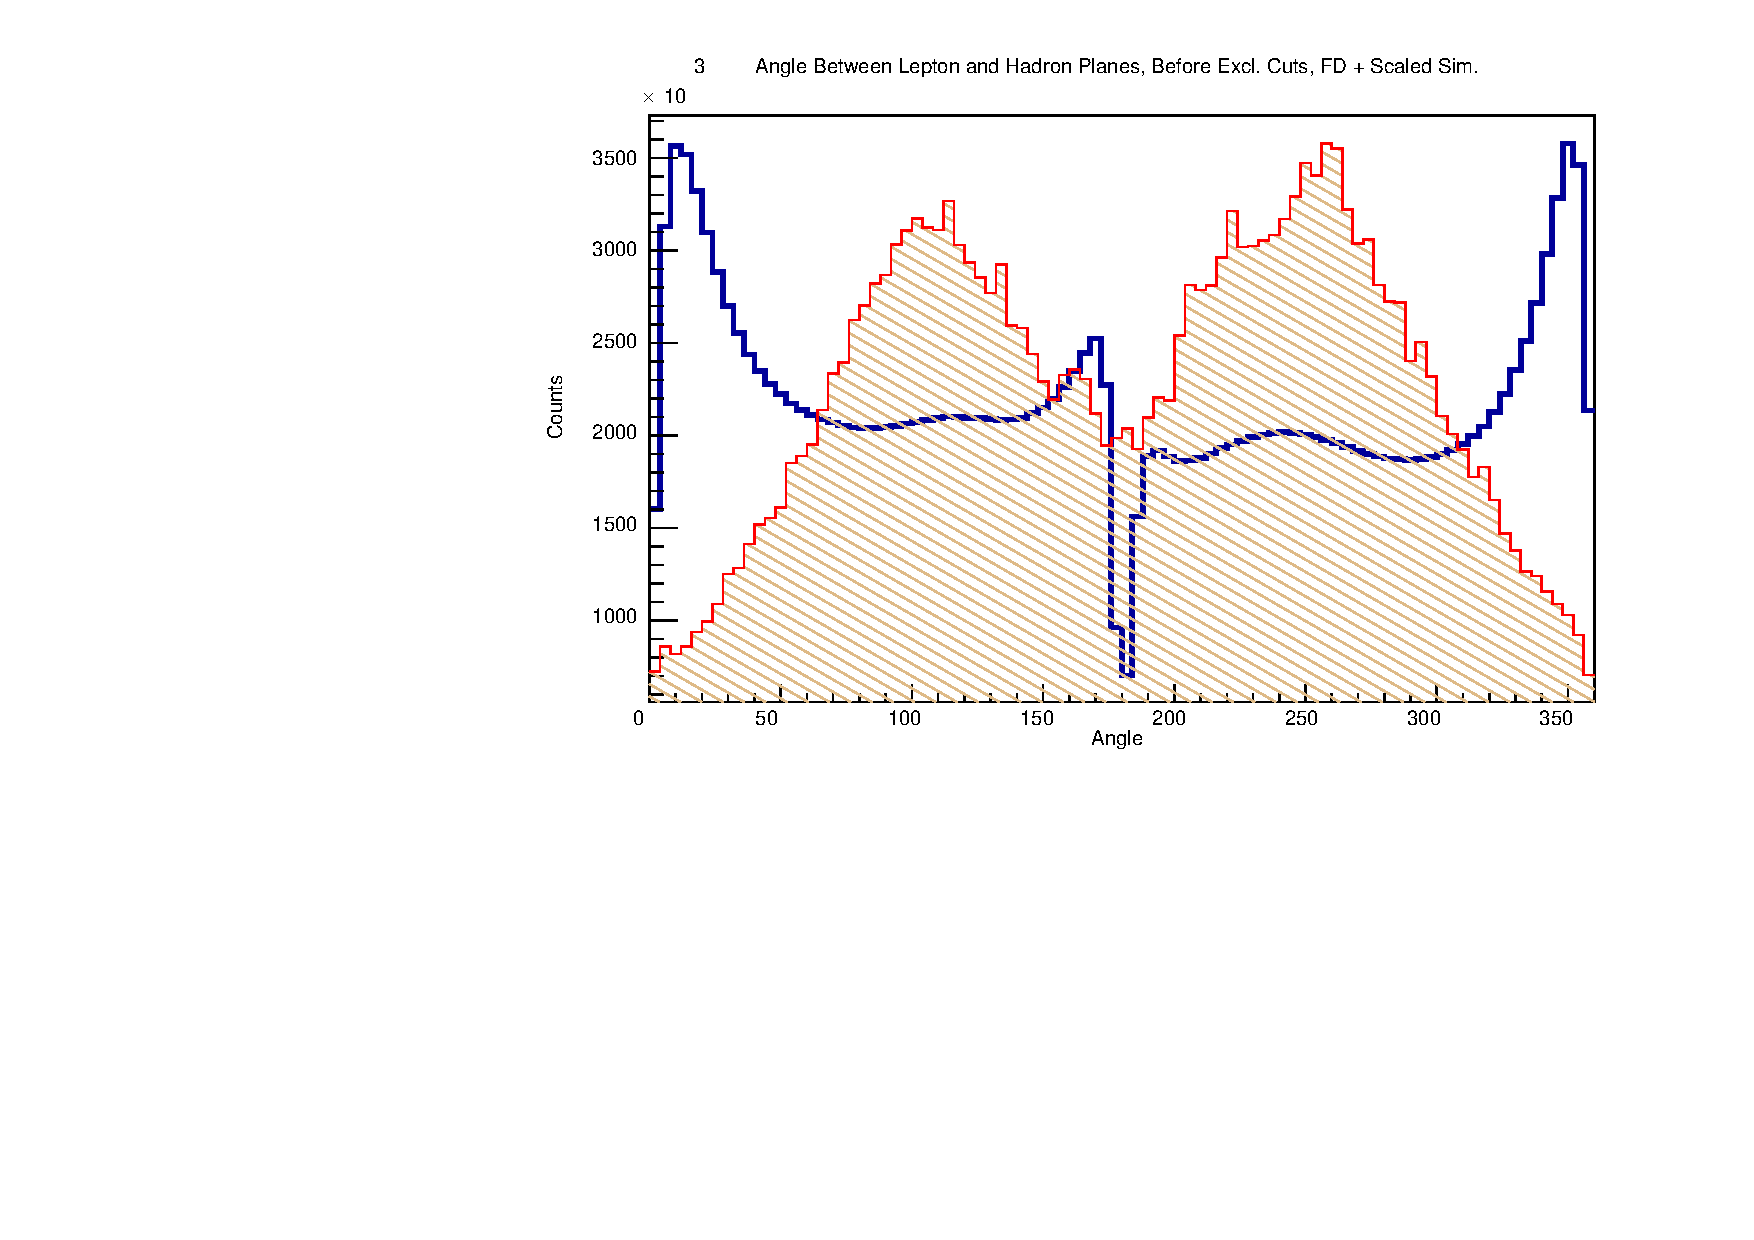
\includegraphics[width=1\textwidth]{figures/Simulation/exclusivity/hist_lept_had_angle_prexcut_fd_Double.pdf}
    \end{subfigure}%
    \begin{subfigure}{.45\textwidth}
        \centering
        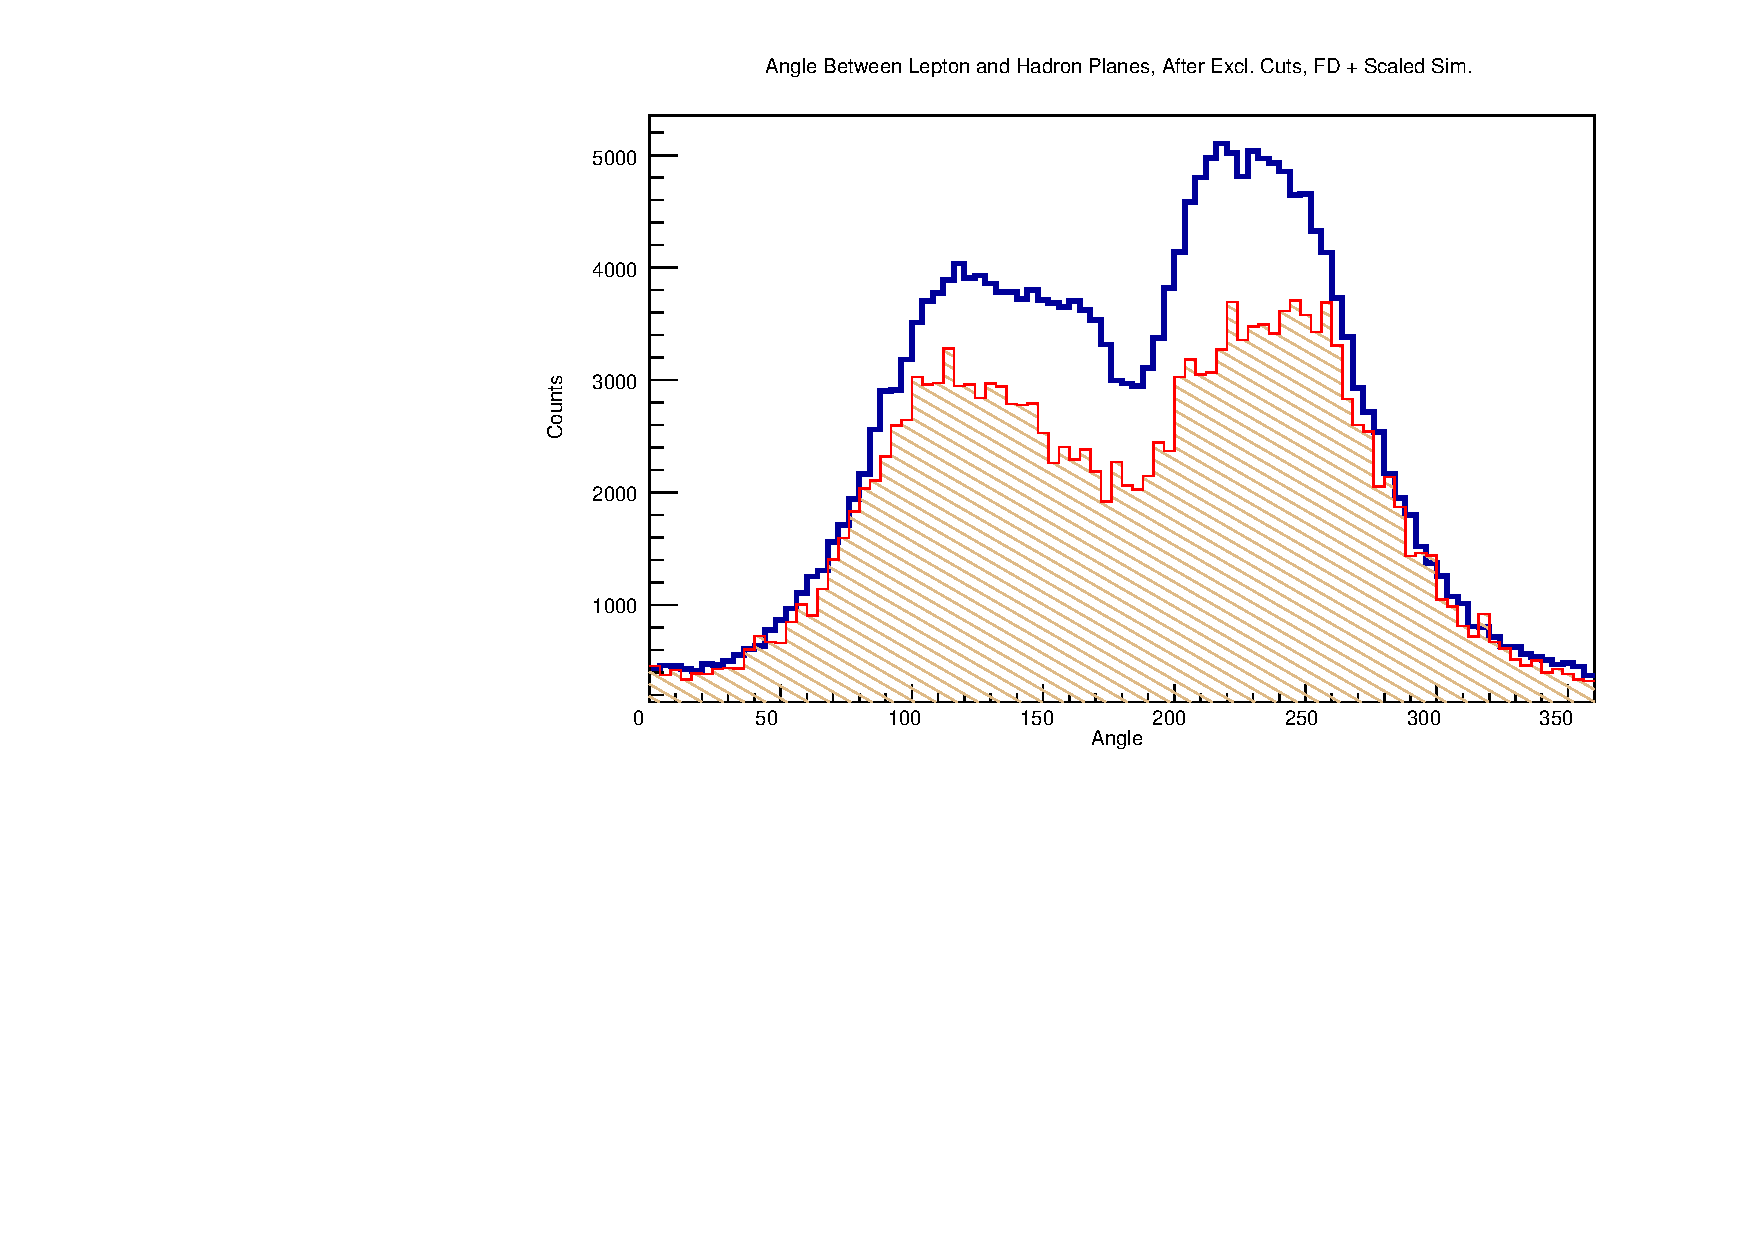
\includegraphics[width=1\textwidth]{figures/Simulation/exclusivity/hist_lept_had_angle_excut_fd_Double.pdf}
    \end{subfigure}
    \caption[short]{Angle between lepton and hadron planes, before exclusivity cuts (left) and after (right) for data (blue) and simulation (red)}
\end{figure}





%\section{Proton PID lookback}
%We extended the analysis to positive tracks.
%Fig.~\ref{fig:finaldatapid} shows the exclusive distributions for positive tracks that were not identified as protons.
%It seems that they are valid exclusive $\pi^0$ electroproduction events even though the positive track was not identified as proton.
%Most of the misidentified tracks happen to be reconstructed in Central Detector.
%Based of Fig.~\ref{fig:finaldatapid} we can make a conclusion that exclusive cuts that we are able to apply because of detection of all final state particles allow us to clean up our sample even without proton PID cuts on positive tracks.
%There seems to be more background for the events with misidentified proton so the tracking improvements (central in particular) would help to clean up the sample in the future.

%\begin{figure}[h]
%    \centering
%    \includegraphics[page=3,width=0.4\linewidth]{figures/eppi0_misc.pdf}
%    \includegraphics[page=4,width=0.4\linewidth]{figures/eppi0_misc.pdf}
%\caption{On the left: is the distribution of $MM^2_{epX}$ for non-proton positive tracks that would pass exclusivity cuts.
%On the right: polar angle for protons in FD (blue), protons in CD (green), non-proton positives in CD (red).}
%    \label{fig:finaldatapid}s
%\end{figure}



%\section{BACKUP}
%\noindent

%\begin{tcolorbox}
%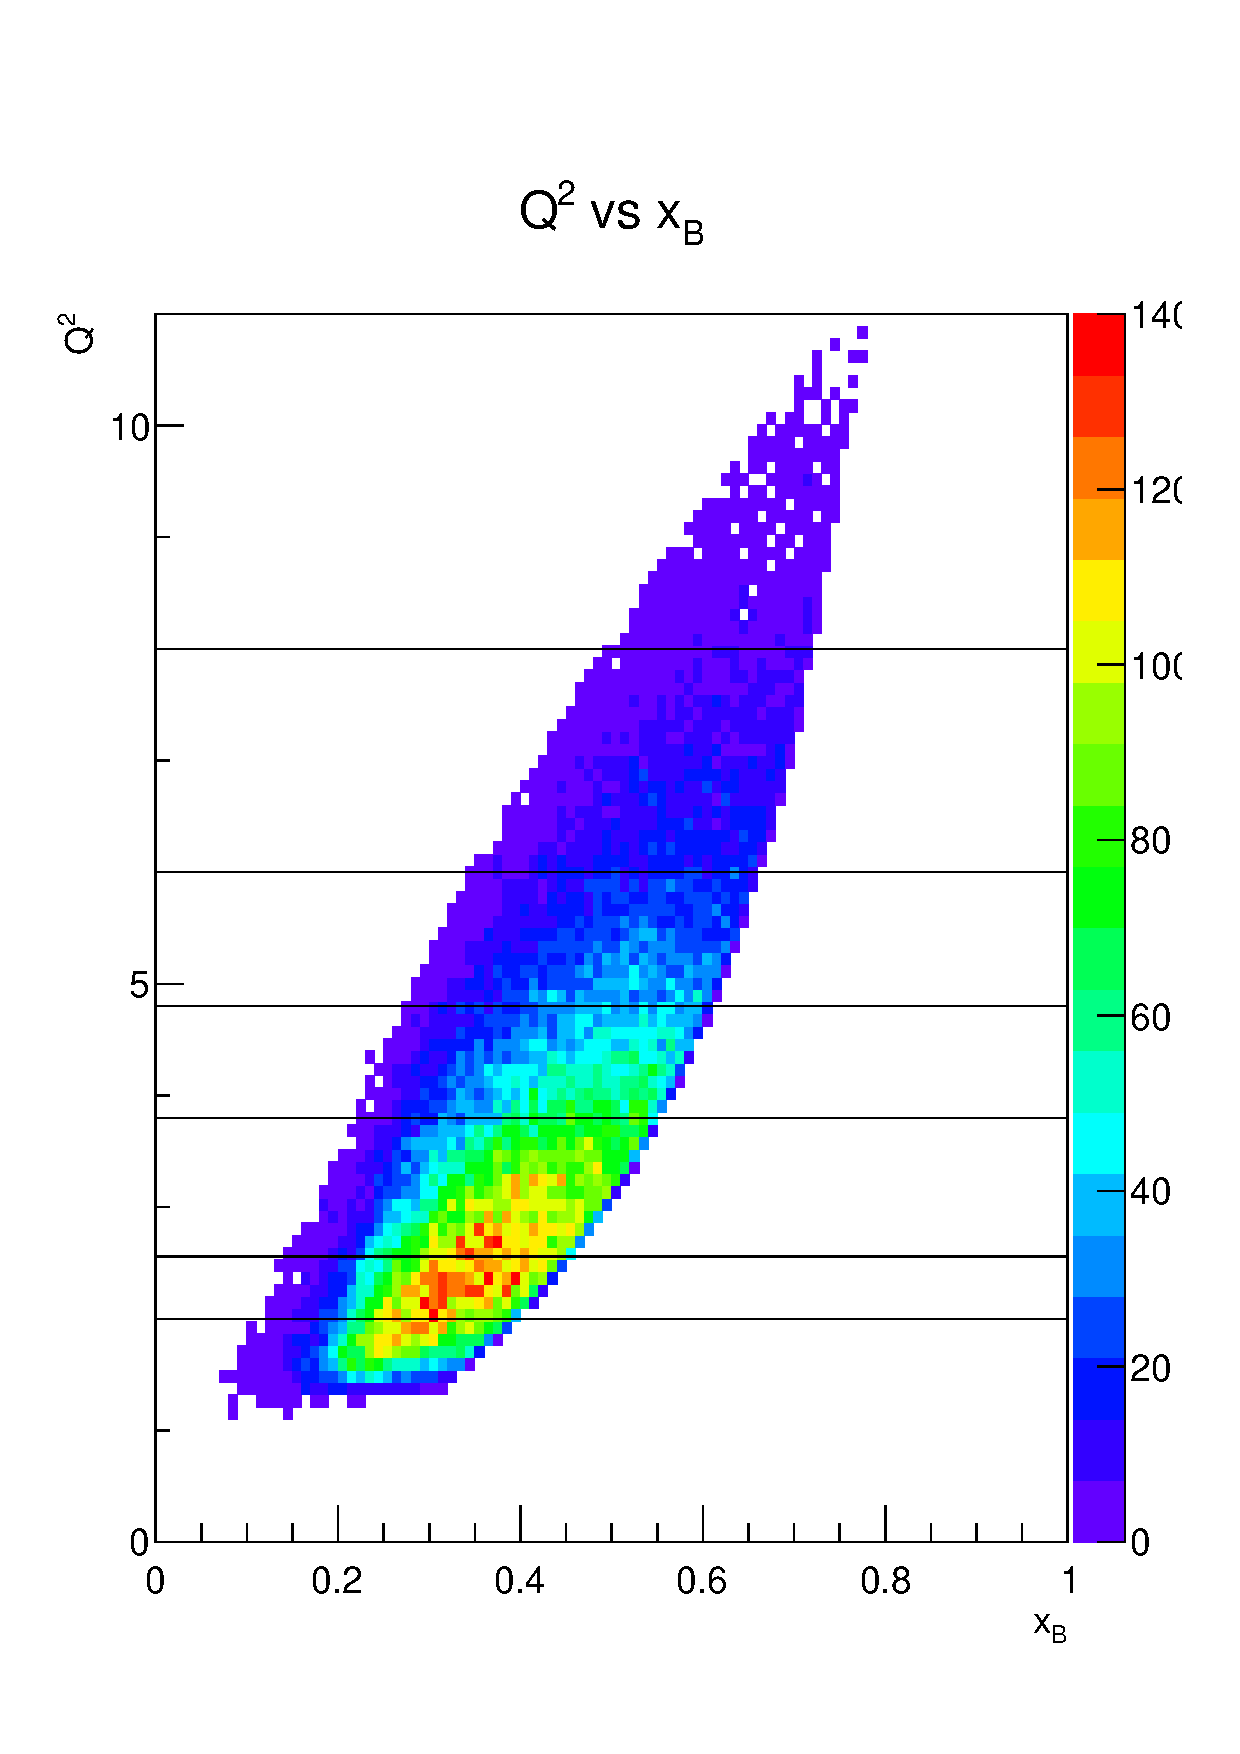
\includegraphics[page=1,width=0.48\linewidth]{figures/bsa_eppi0_ge_pro_fd.pdf}
%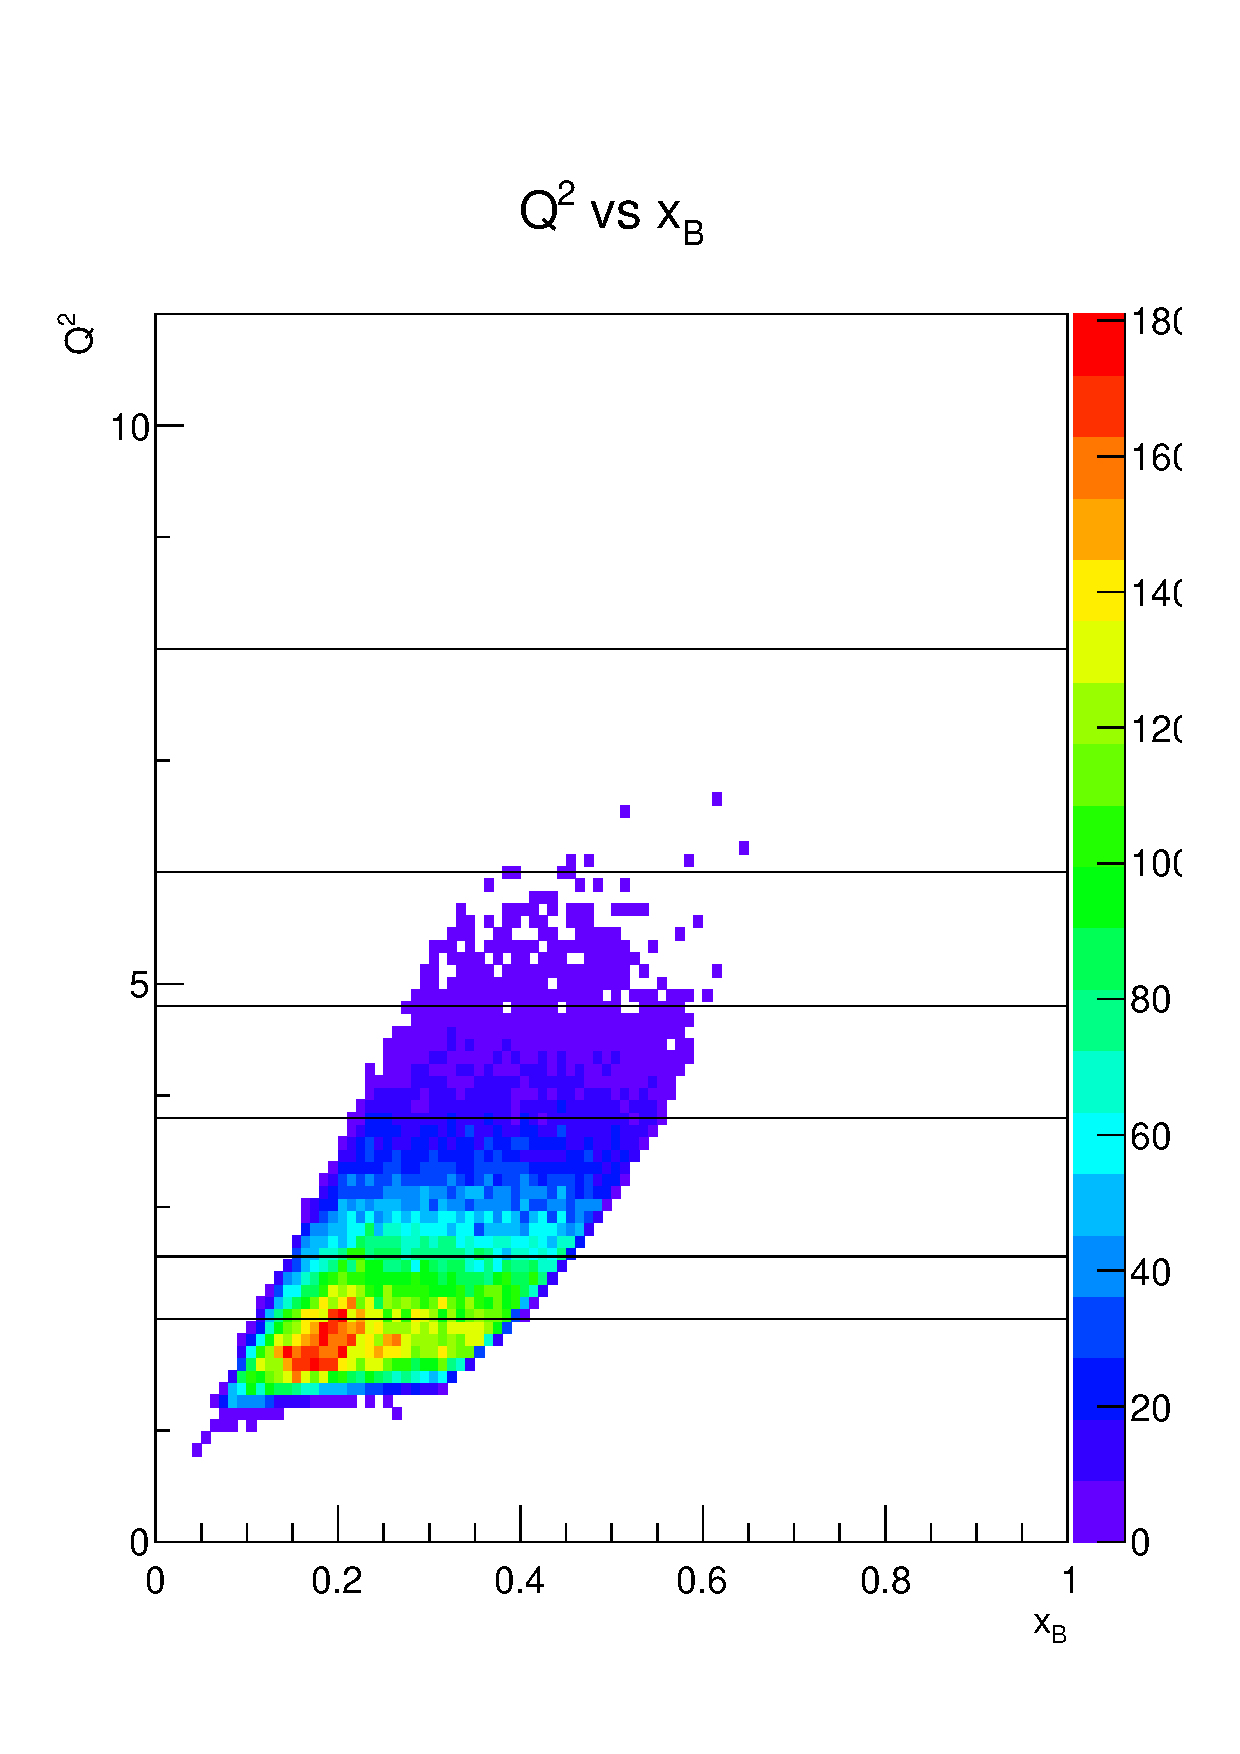
\includegraphics[page=1,width=0.48\linewidth]{figures/bsa_eppi0_ge_pro_cd.pdf}
%\end{tcolorbox}

%\begin{tcolorbox}
%\includegraphics[page=2,width=0.48\linewidth]{figures/bsa_eppi0_ge_pro_fd.pdf}
%\includegraphics[page=2,width=0.48\linewidth]{figures/bsa_eppi0_ge_pro_cd.pdf}
%\end{tcolorbox}

%\begin{tcolorbox}
%\includegraphics[page=3,width=0.48\linewidth]{figures/bsa_eppi0_ge_pro_fd.pdf}
%\includegraphics[page=3,width=0.48\linewidth]{figures/bsa_eppi0_ge_pro_cd.pdf}
%\end{tcolorbox}

%\begin{tcolorbox}
%\includegraphics[page=4,width=0.48\linewidth]{figures/bsa_eppi0_ge_pro_fd.pdf}
%\includegraphics[page=4,width=0.48\linewidth]{figures/bsa_eppi0_ge_pro_cd.pdf}
%\end{tcolorbox}

%\begin{tcolorbox}
%\includegraphics[page=5,width=0.48\linewidth]{figures/bsa_eppi0_ge_pro_fd.pdf}
%\includegraphics[page=5,width=0.48\linewidth]{figures/bsa_eppi0_ge_pro_cd.pdf}
%\end{tcolorbox}

%\begin{tcolorbox}
%\includegraphics[page=6,width=0.48\linewidth]{figures/bsa_eppi0_ge_pro_fd.pdf}
%\includegraphics[page=6,width=0.48\linewidth]{figures/bsa_eppi0_ge_pro_cd.pdf}
%\end{tcolorbox}

%\begin{tcolorbox}
%\includegraphics[page=7,width=0.48\linewidth]{figures/bsa_eppi0_ge_pro_fd.pdf}
%\includegraphics[page=7,width=0.48\linewidth]{figures/bsa_eppi0_ge_pro_cd.pdf}
%\end{tcolorbox}

